\documentclass{article}
\usepackage[%
    left=0.5in,%
    right=0.5in,%
    top=0.5in,%
    bottom=0.5in,%
]{geometry}%
\usepackage{minitoc}
\usepackage{graphicx}
\graphicspath{ {./} }

\begin{document}
\section{Process scheduling}

\subsection{Context}
\begin{flushleft}
The OS is responsible for \textbf{managing} and \textbf{scheduling processes}. It has to decide
\begin{itemize}
	\item When to \textbf{admin} processes to the system (new -> ready)
	\item Which process to \textbf{run} next (ready -> run)
	\item When and which processes to \textbf{interrupt} (running -> ready)
\end{itemize}
It relies on the \textbf{scheduler} (dispatcher) to decide which process to run next, which uses \textbf{scheduling algorithm} to do so

The type of algorithm used by the scheduler is influenced by the the \textbf{type of the operating system} (e.g. real time vs. batch)
\end{flushleft}

\subsection{Classification by Time Horizon}
\begin{flushleft}
\textbf{Long term:} applies to \textbf{new processes} and controls the degree of multiprogramming by deciding which processes to admit to the system when
\begin{itemize}
	\item A good \textbf{mix} of \textbf{CPU} and \textbf{I/O bound processes} is favourable to keep all resources as busy as possible
	\item \textbf{Usually absent} in popular/modern OS
\end{itemize}

\textbf{Medium term}  controls swapping and the degree of multi-programming

\textbf{Short term}: decide which process to run next
\begin{itemize}
	\item Manages the \textbf{ready queue}
	\item Invoked very \textbf{frequently}, hence must be \textbf{fast}
	\item Usually called in response to \textbf{clock interrupts, I/O interrupts, or blocking system calls}
\end{itemize}
\end{flushleft}

\subsection{Classification by Approach}
\begin{flushleft}
\textbf{Non-preemptive:} processes are only interrupted voluntarily (e.g., I/O operations or "nice" system call - yield()). Windows 3.1 and DOS were non-preemptive

\textbf{Preemptive} processes can be \textbf{interrupted forcefully or voluntarily}
\begin{itemize}
	\item This requires context switches which generate \textbf{overhead}, too many of them should be avoided
	\item Prevents processes from \textbf{monopolising the CPU}
	\item \textbf{Most popular} modern operating systems are preemptive
\end{itemize}
\end{flushleft}

\section{Performance Assesment}

\subsection{Criteria}
\begin{flushleft}
\textbf{User oriented criteria:}
\begin{itemize}
	\item \textbf{Response time} minimise the time between creating the job and its first execution
	\item \textbf{Turnaround time} minimise the time between creating the job and finishing it
	\item \textbf{Predictability time} minimise the variance in processing times
\end{itemize}

\textbf{System oriented criteria:}
\begin{itemize}
	\item \textbf{Throughput:} maximise the number of jobs processed per hour
	\item \textbf{Fairness:} Are the processing power/waiting time equally distributed. Are some processes kept waiting execessively long (\textbf{starvation})
\end{itemize}
Evaluation criteria can \textbf{conflicting} i.e, \textbf{improving the response time} may require \textbf{more context switches}, and hence \textbf{worsen the throughout} and \textbf{increase the turn around time}
\end{flushleft}

\section{Scheduling algorithms}

\subsection{Overview}
\begin{flushleft}
\textbf{Algorithms} considered
\begin{itemize}
	\item First come first served \textbf{FCFS}/ First in first out \textbf{FIFO}
	\item \textbf{Shortest job first}
	\item \textbf{Round robin}
	\item \textbf{Priority queues}
\end{itemize}
Performance measure used:
\begin{itemize}
	\item \textbf{Average response time}: the average of the time taken for all the processes to start
	\item \textbf{Average turnaround time}: the average time taken for all the processes to finish
\end{itemize}
\end{flushleft}

\subsection{First come first served FCFS}
\begin{flushleft}
Concept: a \textbf{non-preemtive algorithm} that operates as a \textbf{strict queueing mechanism} and schedules the processes in the same order that they were added to the queue\\
Advantages: \textbf{positional fairness} and easy to implement\\
Disadvantages:
\begin{itemize}
	\item \textbf{Favours long processes} over short ones
	\item Could \textbf{compromise resource utilisation}, i.e., CPU vs I/O devices
\end{itemize}
\end{flushleft}

\begin{center}
  \makebox[\textwidth]{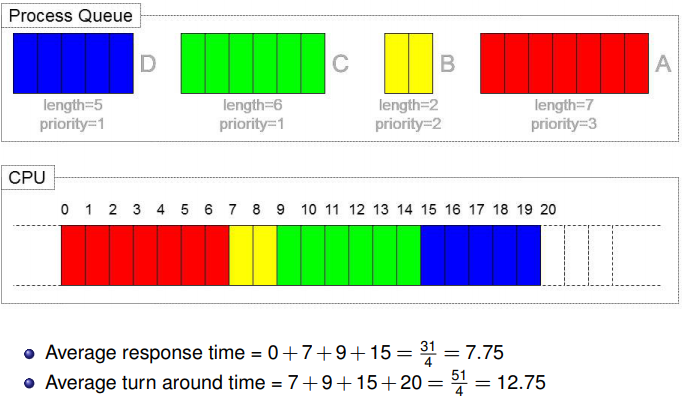
\includegraphics[scale=0.5]{FCFS.png}}
\end{center}
\pagebreak

\subsection{Shortest job first}
\begin{flushleft}
Concept: a \textbf{non-preemtive algorithm} that starts processes in order of
\textbf{ascending processing time}using a provided/known estimate of the processing\\
Advantages: always result in the \textbf{optimal turn around time}\\
Disadvantages:
\begin{itemize}
	\item \textbf{Starvation} may occur
	\item \textbf{Fairness} and \textbf{predictability} are compromised
	\item \textbf{Processing times have to be known} beforehand
\end{itemize}
\end{flushleft}
\begin{center}
  \makebox[\textwidth]{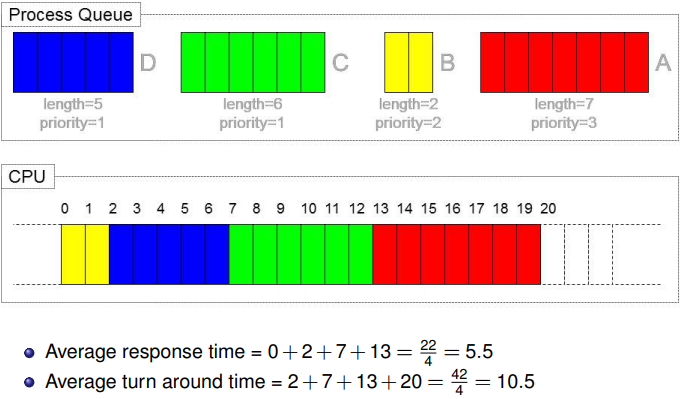
\includegraphics[scale=0.5]{Selection_002.png}}
\end{center}

\subsection{Round robin}
\begin{flushleft}
Concept: a \textbf{preemptive version of FCFS} that forces \textbf{context switches} at \textbf{periodic intervals or time slices}
\begin{itemize}
	\item Processes \textbf{run in order that they were added} to the queue
	\item Processes are forcefully \textbf{interrupted by the timer}
\end{itemize}
Should be used when it is desirable to allow long running processes to execute while not interfering with shorter ones
Advantages:
\begin{itemize}
	\item Improved \textbf{response time}
	\item Effective for general purpose \textbf{time sharing systems}
	\item Starvation free
\end{itemize}
Disadvantages:
\begin{itemize}
	\item Increased \textbf{context switching} and thus overhaul
	\item \textbf{Favours CPU bound processes}(which usually run long) over I/O (which do not run long). Can be prevented by working with multiple queues
	\item Can \textbf{reduce to FCFS}
\end{itemize}
The lenght of time \textbf{time slice} must be carefully considered\\
For instance, assuming a \textbf{multi-programming system} with \textbf{preemptive scheduling} and a \textbf{context switch time of 1ms}\\
\begin{itemize}
	\item A \textbf{good (low) response time} is achieved with a \textbf{small time slice}(1ms) => low throughput
	\item A \textbf{hight throughput} is achieved with a \textbf{large time slice} (1000ms) => hight response time
\end{itemize}
If a time slice is only \textbf{used partially} the next process \textbf{starts immediately}
\end{flushleft}
\begin{center}
  \makebox[\textwidth]{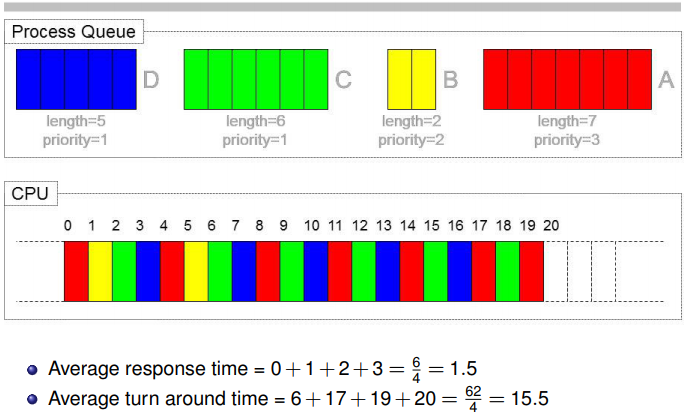
\includegraphics[scale=0.5]{Selection_003.png}}
\end{center}

\subsection{Priority queues}
\begin{flushleft}
Concept: A \textbf{preemptive algorithm} that schedules processes by priority (high => low). The process priority is saved in the \textbf{process control block}\\
Advantages: can \textbf{prioritise I/O bound jobs}\\
Disadvantages: low priority processes may suffer from \textbf{starvation} with static priorities.
\end{flushleft}
\begin{center}
  \makebox[\textwidth]{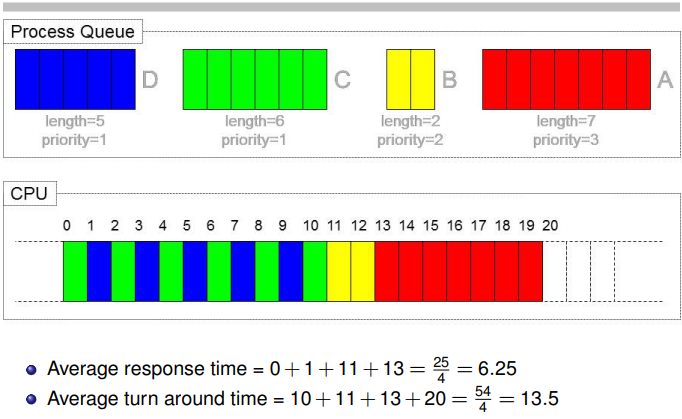
\includegraphics[scale=0.5]{Selection_005.png}}
\end{center}

\section{Summary}
\begin{itemize}
	\item The OS is responsible for \textbf{process scheduling}
	\item Different types of schedulers exist
	\item Different \textbf{evaluation criteria} exists for process scheduling
	\item Different \textbf{algorithms} should be considered
\end{itemize}
\end{document}